\section{Parties bornées d'un éspace métrique}
\begin{definition}
    Une partie $A \subset E$ est bornée s'ils existent $x_0 \in E$ et  $r > 0$ tels que  $A \subset B(x_0, r)$
\end{definition}
\begin{prop}
    S'il existe $r > 0$ tel que $\forall x, y \in A, \, d(x, y) \le r$, alors $A$ est bornée.
\end{prop}
\begin{definition}
    La distance entre deux ensembles $A, B$ est:
     \[
         d(A, B) := \underset{x \in A, y \in B}{inf}d(x, y)
    \] 
    Intuitivement, on cherche deux points $x$ et  $y$ tel que la distance est la plus petite possible.
\end{definition}
\begin{definition}
    La distance entre un points $x$ et un ensemble  $B$ est:
     \[
         d(x, B) := \underset{y \in B}{inf}d(x, y)
    \] 
    La même intuition.
\end{definition}
\section{Topologie des éspaces métriques}
\begin{definition}
    .
    \begin{enumerate}
        \item Un ensemble $U \subset  E$ est \textbf{ouvert} si $\forall x \in U$ $\exists \delta > 0$ tel que $B(x, \delta) \subset U$.
        \item Un ensemble $F \subset E$ est \textbf{fermé} si $E \setminus F$ est ouvert, i.e $\forall x \in E \setminus F$ $\exists \delta > 0$ tel que $B(x, \delta) \subset E\setminus F$
    \end{enumerate}
\end{definition}
\begin{figure}[H]
    \centering
    \begin{subfigure}{0.45\textwidth}
        \centering 
        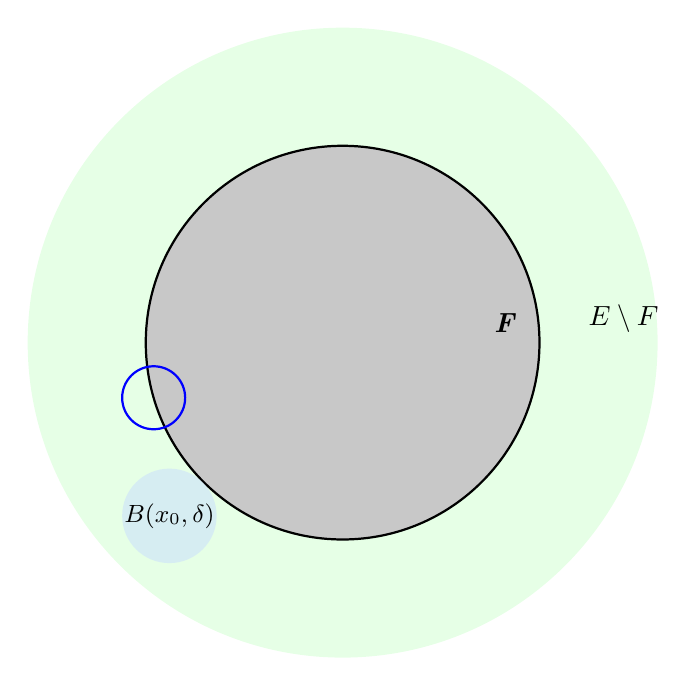
\begin{tikzpicture}
            % Define colors
            \definecolor{lightgreen}{RGB}{230, 255, 230}
            \definecolor{lightblue}{RGB}{200, 220, 255}
            \definecolor{darkgreen}{RGB}{0, 128, 0}

            % Large background circle
            \fill[lightgreen] (0, 0) circle (4cm);

            % Main circle
            \draw[thick, fill=lightgray] (0, 0) circle (2.5cm);
            \node[above right] at (1.8, 0) {\textbf{\textit{F}}};
            \node[above right] at (3, 0) {$E\setminus F$};

            % Small blue circle
            \draw[blue, thick] (-2.4, -.7) circle (0.4cm);

            % Highlighted area for excluded point
            \fill[lightblue, opacity=0.5] (-2.2, -2.2) circle (0.6cm);
            \node (_) at (-2.2, -2.2){\small $B(x_0, \delta)$};
        \end{tikzpicture}
        \caption{Un ensemble fermé\\
            \textit{À la borne, il est impossible de trouver une boules qui appartient à $F$, car il est impossible d'avoir une boule ouverte de  $r = 0$. Exemple: circle bleu foncé}\\
            \textit{Pour tout point dans $E \setminus F$ on peut trouver une boule ouverte}
        }
    \end{subfigure}
    \hfill
    \begin{subfigure}{0.45\textwidth}
        \centering
        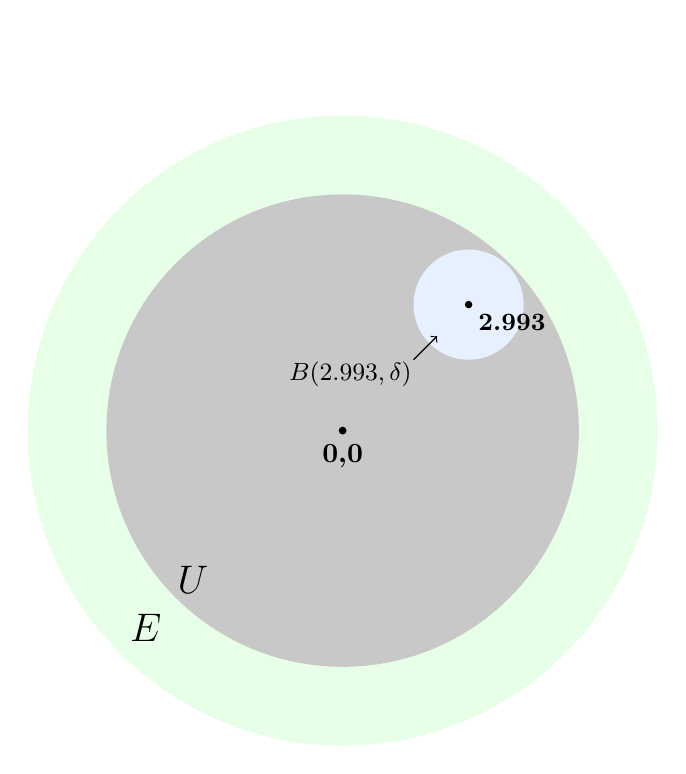
\begin{tikzpicture}
            % Define colors
            \definecolor{lightblue}{RGB}{230, 240, 255}
            \definecolor{lightgray}{RGB}{200, 200, 200}
            \definecolor{darkgreen}{RGB}{0, 128, 0}
            \definecolor{lightgreen}{RGB}{230, 255, 230}

            % Draw large circle
            \fill[lightgreen] (0, 0) circle (4cm);
            \fill[lightgray] (0, 0) circle (3cm);

            % Draw small circle
            \fill[lightblue] (1.6, 1.6) circle (0.7cm);
            \draw[fill=black] (1.6, 1.6) circle(0.4mm);
            \node[below right] at (1.6, 1.6) {\textbf{\small 2.993}};

            \draw[->] (0.9, 0.9)--(1.2, 1.2);
            \node[below left] (_) at (1, 1){\small $B(2.993, \delta)$};
            % Add points and labels
            \node[fill=black, circle, inner sep=1pt, label=below:{\textbf{0,0}}] at (0, 0) {};

            % Add text
            \node[right] at (1, 5) [align=left, text=darkgreen] {
                };
            \node (_) at (-1.9, -1.9){\Large $U$};
            \node (_) at (-2.5, -2.5){\Large $E$};
        \end{tikzpicture} 
        \caption{Un ensemble ouvert\\
            \textit{
                pour tout point pres de la borne
                on peut trouver une boule
                infiniment petite avec des
                points autour ce point inclu dans $U$.
            }
        }

    \end{subfigure}
    \caption{Démonstration des espaces ouverts et fermés}
\end{figure}

\begin{prop}.
    \begin{enumerate}
        \item 
            Une union des ensembles ouverts est aussi ouvert, idem avec l'intersection des ensembles ouverts. 
        \item  
            Une union des ensembles fermé est aussi fermé, idem avec l'intersection des ensembles fermé. 
    \end{enumerate}
\end{prop}

\section{Intérieur, adhérence, frontière}
Soit $A \subset E$. 
\begin{definition}
    Un point $x \in E$ est intérieur à $A$ s'il existe  $\delta > 0$ tel que  $B(x, \delta) \subset A$.\\
    Ensembles des points intérieur à $A$ se note  $Int(A)$ ou  $\mathring{A}$.
\end{definition}
\begin{intuition}
   $Int(A)$ est un ensemble qui est totalement dans  $A$ est se trouve loin des bords. 
\end{intuition}
\begin{tabular}[c]{@{}l@{}r@{}}
    \adjustbox{valign=t}{
    \parbox[t]{0.79\textwidth}{
    \begin{definition}
        Un point $x \in E$ est adhérent à  $A$ si  $\forall r > 0, \, B(x, r) \cap A \neq \O$ (toute boule centré dans $x$ intersecte  $A$).  \\
        Ensemble des points adhérents à $A$ se note  $Adh(A)$ ou  $\overline{A}$.
    \end{definition}
}
}
    &
    \hfill
    \adjustbox{valign=t}{
        \parbox[t]{0.2\textwidth}{
            \vspace{0.3cm}
    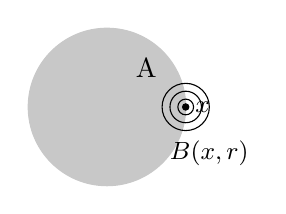
\begin{tikzpicture}
            \definecolor{lightgray}{RGB}{200, 200, 200}
        \filldraw[color=lightgray] (0,0) circle (1cm); 
        \coordinate (x) at (1, 0);
        \filldraw[color=black] (x) circle (0.4mm);
        \node[right] (_) at (x){\small $x$};
        \node (_) at (0.5, 0.5){A};

        \draw (x) circle (0.2cm);
        \draw (x) circle (0.3cm);
        \draw (x) circle (0.1cm);
        \node[below] (_) at (1.3, -0.3){\small $B(x, r)$};
    \end{tikzpicture} 
}
}
\end{tabular}
\begin{intuition}
   Si $A$ est ouvert (ses bords n'appartiennent pas à $A$), ses bords appartiennent à $Adh(A)$. Cette notion est utile pour completer des ensembles.
   \begin{eg}
       $\overline{\Q} = \R$ 
   \end{eg} 
\end{intuition}
\begin{definition}
    $Adh(A) \cap Adh(E \setminus A)$ est le bord de $A$ est s'appelle  la frontière de $A$.
\end{definition}
\section{Suite dans un éspace métrique}
\begin{definition}
    Une suite $(x_n)_{n \in \N}$ converge vers $x \in E$, si  $\forall \epsilon > 0, \exists N \in \N$ tel que :
    \[
    \forall n \ge N, \, d(x_n, x) \le  \epsilon
    \] 
\end{definition}
\begin{prop}
   Soit $A \in E$.\\ 
   \begin{enumerate}
       \item $x \in Adh(A)$ si et seulement si, il existe une suite $(x_n)_{n \in \N}$ d'éléments de $A$ telle que  $x_n \xrightarrow[n \to +\infty]{} x$ 
       \item $A$ est fermé (i.e contient sa frontière) si et seulement si la limite de toute suite  $(x_n)_{n \in \N}$ d'éléments de $A$ appartient à  $A$.
   \end{enumerate}
\end{prop}
\begin{intuition}
   \begin{enumerate}
       \item Si $(x_n)_{n \in \N}$ est d'éléments de  $A$ ($\forall n \in N, \, x_n \in A$), donc elle converge vers un éléments $x$ qui peut être soit dans  $A$, soit la borne des éléments de  $A$, alors à la frontière. 
       \item Si la limite de toute suite $(x_n)_{n \in \N}$ des éléments de  $A$ est aussi dans  $A$, alors la frontière de  $A$ est inclu dans  $A$. Car l'une des suites tend vers la borne.
   \end{enumerate} 
\end{intuition}
\begin{definition}
    Une suite $(x_n)_{x \in \N}$ est de Cauchy si  $\forall \epsilon > 0, \exists N \in \N$ tel que:
    \[
    \forall n, p \ge N, \, d(x_n, x_p) \le \epsilon
    \] 
\end{definition}
\begin{intuition}
   Une suite de Cauchy c'est comme on mesure un point et on le localise, i.e:
   \begin{enumerate}
       \item On dit qu'il est entre $0$ et  $1$.
       \item Ensuite, on precise plus et on dit qu'il est entre  $0.5$ et  $0.6$.
       \item Puis, entre  $0.55$ et  $0.56$
   \end{enumerate}
   On peut infiniment augmenter le niveau de précision. C'est ça l'idée d'une suite de Cauchy.
\end{intuition}
\begin{definition}
    Un éspace métrique $(E, d)$ est \textbf{complet} si toute suite  $(x_n)_{n \in \N}$ d'éléments de  $E$ converge vers une limite  $x$ qui appartient aussi à  $E$.
\end{definition}
\begin{eg}
    Un éspace métrique $(]0, 1], d)$ avec $d$ une distance euclidienne n'est pas complet, car  soit une suite: $x_n = \frac{1}{n}$ dont la limite est $0$. Par contre,  $0 \not\in ]0, 1]$. Donc cet éspace n'est pas complet. 
\end{eg}
\begin{figure}[h]
   \centering 
   \begin{tikzpicture}
       \draw[->] (-1, 0) -- (2, 0); 
       \node[below] (_) at (2,0){$x$};

       \node (_) at (0,0){]};
       \node[below] (_) at (0,-0.3){$0$};
       \node (_) at (1,0){]};
       \node[below] (_) at (1,-0.3){$1$};
       \draw[color=red] (0,0)--(1,0);
   \end{tikzpicture}
   \caption{$(]0, 1], d)$ n'est pas complet}
\end{figure}
\begin{eg}
   Un éspace $(\Q, d)$ n'est pas complet. Car on peut prendre une suite  $x_n$ tendant vers  $\sqrt{2} \not\in \Q$.
\end{eg}

\begin{figure}[H]
    \centering
    \incfig{q_not_complete}
    \caption{$\Q$ pas complet}
    \label{fig:q_not_complete}
\end{figure}

\begin{definition}
    Soit une suite $(x_n)_{n \in \N}$ et une application  $\phi:\N \to \N$ \underline{strictement croissante}. Une suite $(x_n)_{\phi(n)}$ est appellée une sous-suite.
\end{definition}
\begin{eg}
    Soit une application $\phi: \N \to \N$ telle que $\phi(n) = 2n$. Donc  $(x_n)_{\phi(n)}$ est une sous-suite de  $(x_n)_{n \in \N}$ et:
    \[
        (x_n)_{\phi(n)} = \{x_0, x_2, x_4, \ldots\}
    \] 
\end{eg}

\section{Compacité}
\begin{definition}
    Soit $F \subset E$. Un \textbf{recouvrement ouvert} de $F$, est une union des enesembles ouverts:  $\bigcup_{i \in I} U_i$ tel que $F \subset \bigcup_{i \in I} U_i$
\end{definition}
\begin{eg}
    Soit $F = ]0, 1[$. Soit $A = \left\{]\frac{1}{n}, 1 + \frac{1}{n}[, n \in N\right\}$. $F \subset \bigcup_{n \in N^{*}} A_n$ i.e union infinie des $A_i$ couvre $F$.
\end{eg}
\begin{definition}
    Un ensemble $F \subset E$ est \textbf{compact} si \underline{pour tout} recouvrement ouvert, i.e \underline{pour tout} union des ensembles ouvert $\bigcup_{i \in I} U_i$ qui couvre $F$, on peut prendre un nombre \underline{fini} des  $U_i$ et couvrir $F$.
\end{definition}
\begin{theorem}
    Un ensemble $K \subset E$ est compact, si toute suite $(x_n)_{n \in \N}$ des éléments de $K$, possede une sous-suite qui converge  vers un éléments $x \in K$.
\end{theorem}
\begin{intuition}
    S'il existe tel suite $(x_n)_{n \in \N}$ sans sous-suite convergente vers un éléments de  $K$, donc les valeurs sont en-dehors de  $K$ et donc il existe un ensemble qui couvre $K$  seulement avec un nombre infini des ensembles. 
\end{intuition}
Pourquoi a-t-on besoin de compacité? Car cela nous donne une
\begin{prop}
    Si $K \subset E$ est compact, alors $K$ est fermé et borné.\\
    Si $K$ est compact est  $F$ est borné, donc  $K \cap F$ est compact\\
    Si $K$ est compact, donc  $K$ est complet
\end{prop}
\begin{property}
    La différence entre \textit{compacité} et {complecité}:
    \begin{itemize}
        \item complecité nous assure qu'il n'y a pas de trou dans un espace
        \item compacité nous assure qu'un ensemble est fermé et borné
    \end{itemize}
\end{property}

